\documentclass{article}

\usepackage[margin=1in]{geometry} % Set margins to 1 inch
\usepackage{graphicx} % Allows including images
\usepackage{float} % Allows for precise placement of figures
\usepackage{amsmath} % Allows for math equations
\usepackage{siunitx} % Allows for SI units
\usepackage{placeins} % Makes sure images are in their respective sections by \FloatBarrier

\begin{document}

\title{Software Assignment Report}
\author{Anagha Balaji \\ EE22BTECH11204}
\date{}
\maketitle

\maketitle

\section{Aim}
To make a python script which can make a playlist of songs and shuffle them.

\section{Introduction}
The provided code implements an audio player using the Pygame library in Python. It allows users to play, pause, skip to the next track, go back to the previous track, and quit the application. The player loads audio files from a specified directory and supports playback of MP3 files.

\section{Overview}
The code begins by importing the necessary modules, including os and pygame. It then sets the path to the directory containing the audio files and initializes the Pygame mixer.
\\
Next, it retrieves a list of audio files in the specified directory, filtering only the ones with the ".mp3" extension. The code also initializes a variable for the current song index.
\\
The play$_$current$_$song() function is defined to load and play the current song. It utilizes the pygame.mixer.music module to load the audio file and start playback. The function also prints the name of the current song.
\\
The initial song is played by calling the play$_$current$_$song() function. Afterward, a while loop is used to repeatedly prompt the user for commands via the input() function.\\
\\
Inside the loop, the user's command is obtained and matched against several possibilities. If the command is "pause", the player pauses the currently playing song using pygame.mixer.music.pause(). If the command is "play", the player resumes playback using pygame.mixer.music.unpause(). For "next" and "prev" commands, the current song index is incremented or decremented, respectively, and the player stops the current song and calls play$_$current$_$song() again with the updated index.
\\
The loop continues until the user enters the "quit" command. In this case, the current song is stopped, and the loop is exited, ending the program.

\section{Conclusion}
The provided code offers a basic audio player that allows users to control playback, skip between tracks, and quit the application. It utilizes the Pygame library to handle audio playback in an efficient and straightforward manner. The code can be extended and customized further to include additional features, such as shuffle or repeat modes, volume control, or a graphical user interface.

\section{Terminal}

\begin{figure}[ht]
        \centering
        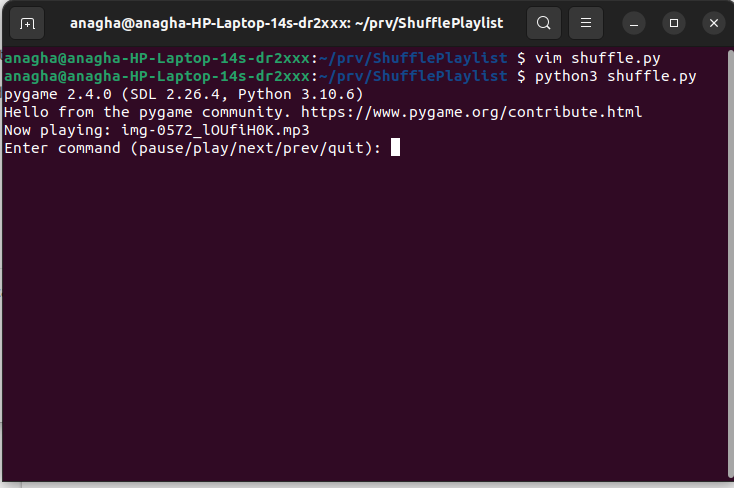
\includegraphics[width=0.8\linewidth]{terminal1.png}
        \caption{}
        \label{fig:view}
\end{figure}

\begin{figure}[ht]
        \centering
        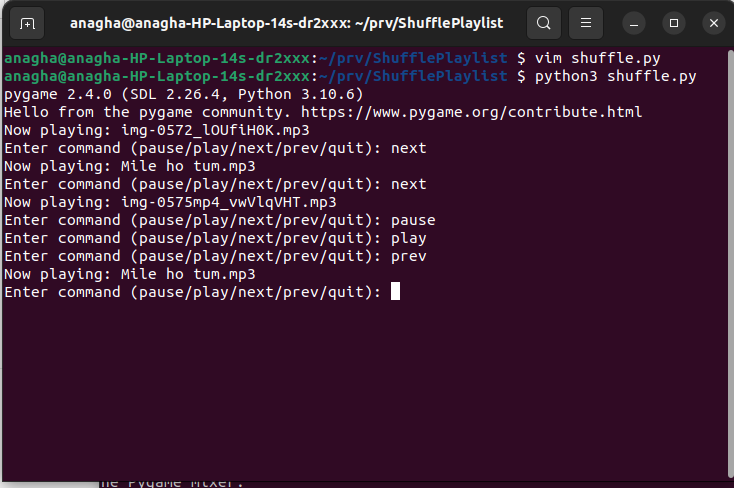
\includegraphics[width=0.8\linewidth]{terminal2.png}
        \caption{}
        \label{fig:view}
\end{figure}

\end{document}
